\section{The Basics of Nuclear Fusion and Tritium Breeding}\label{sec:fusion-basics}
The controlled, sustained thermonuclear fusion of light elements is the ultimate energy source for humanity. Fusion is an energy source that is inexhaustable (on our planetary scales), produces none of the greenhouse gases that are altering the climate of our planet in potentially devastating ways, and avoids many of the dangers of nuclear fission. But overcoming the engineering obstacles to tame the fusion reaction is the greatest technological challenge of our generation.

The most favorable fusion reaction for first generation fusion reactors involves the two hydrogen isotopes of deuterium and tritium. The deuterium-tritium (DT) reaction has a high reaction probability at the lowest ion temperature with high energy yield. Alternative fusion reactions of two deuterium atoms or a deuterium atom with helium-3 are advantageous in other regards, such as no radioactive byproducts or fuel availability, but their relatively higher ion temperature preclude them from current consideration. The DT reaction proceeds as
\begin{align}
	\mathrm{D} + \mathrm{T}&\xrightarrow{}~^4\mathrm{He}+\mathrm{n}+17.58~\text{MeV} \label{eq:dt-reaction}
\end{align}

Of the two isotopes fused, deuterium ($D$, or $^2$H) is a stable isotope and is naturally occuring in an average abundance of 0.015 mole percent in water on Earth. To demonstrate just how plentiful deuterium is as a fuel source, there is approximately 100 million billion kilograms of deuterium in the Earth's oceans. If all energy on Earth were produced from DT fusion power plants, there would be enough deuterium to outlast the lifetime of our sun. We will not run out of peak deuterium.  

Tritium ($T$, or $^3$H), however, is radioactive with a half-life of only about 12.32 years; any naturally occurring tritium decays at such a rapid pace it will never accumulate to an appreciable amount on Earth. If tritium is to be used as a fuel in a fusion power plant, it must be generated artificially. 

A method of in-situ generation of tritium in a fusion reactor is to include a so-called tritium breeding blanket that surrounds the plasma with a phase of lithium. Natural lithium will interact with neutrons as
\begin{subequations}\label{eq:lithium-t}
\begin{align}
	\mathrm{n} + ~^7\mathrm{Li} &\xrightarrow ~\mathrm{n}+\alpha + \mathrm{T} -2.47~\text{MeV}\label{eq:li7-t}\\
	\mathrm{n} + ~^6\mathrm{Li} &\xrightarrow ~ \alpha + \mathrm{T} +4.78~\text{MeV} \label{eq:li6-t}
\end{align}
\end{subequations}
where we haved used the common short-hand of $\alpha$ in place of the helium nucleus. The cross-sections of the lithium reactions are given in Fig.~\ref{fig:li-xsects}. Note the exothermic lithium-6 reaction (a neutron of any energy will incite the transmuation) and the threshold energy required of the incident neutron in the endothermic lithium-7 reaction.

\begin{figure}
	\centering
	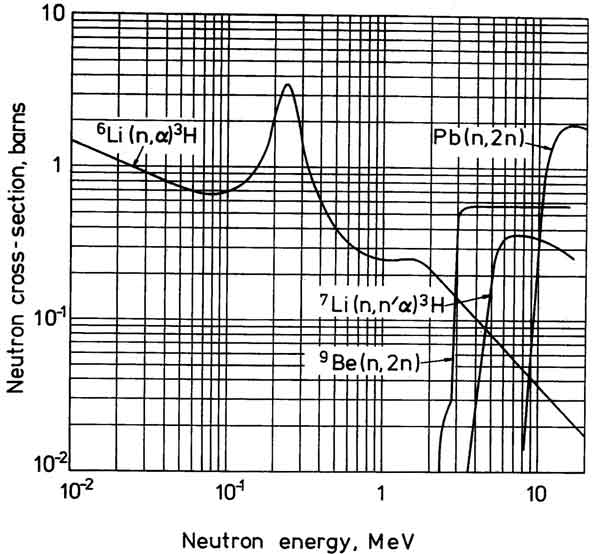
\includegraphics[width=0.75\textwidth]{chapters/figures/breeding_xsecs} 
	\caption{Cross-sections of various blanket materials. Note the threshold for the $^7$Li and neutron multiplying reactions.}
	\label{fig:li-xsects}
\end{figure}

Lithium, like deuterium, is quite abundant on Earth. As noted in Francis Chen's book on the fusion, there is enough lithium available on land to generate tritium for 30 million years of DT reactions providing all of humanity's electricity.\cite{chens-textbook}. 

To reiterate, neither the fusion reaction of Eq.~\ref{eq:dt-reaction} nor the necessary transmutations of lithium in Eqs.~\ref{eq:lithium-t} produce any greenhouse gases. The nature of fusion requires a constant supply of fuel (and extremely careful engineering) to keep the plasma burning; there is no risk of the fusion reactor going into melt-down. For even the first generation fusion reactors, the necessary fuel will last beyond the timeline of humanity on Earth. Furthermore, the next generation fusion reactors will likely move away from tritium and will have virtually no concern of radioactive waste. Fusion power is unarguably the ultimate energy source for humans on Earth and, if we continue to live the lives of comfort we currently enjoy, is in absolutely critical step in humanity's march forward.

% \begin{figure}
% 	\centering
% 	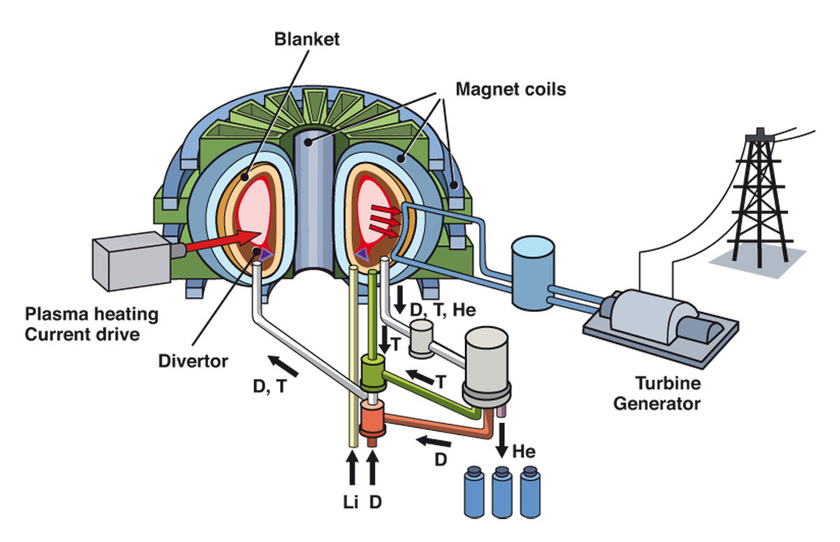
\includegraphics[width=0.85\textwidth]{chapters/figures/power-plant-schematic} 
% 	\caption{Schematic of a tokamak power plant showing the role of the blanket in both energy production and tritium breeding. (reproduced from the Max-Planck-Institut für Plasmaphysik)}
% 	\label{fig:power-plant-schematic}
% \end{figure}

% In Fig.~\ref{fig:power-plant-schematic}, a schematic of a potential magnetically-confined fusion power plant is shown. In the illustration, we see the blanket surrounding the toroidally-shaped plasma and how the tritium generated in the blanket is recycled on-site to be fed back into the burning plasma. Also apparent in the sketch is the role of the breeding blanket as power generator. In \cref{sec:blanket-design}, we will go into more detail on the complete function of a breeding blanket in a fusion reactor.
